\documentclass{article}
\usepackage[utf8]{inputenc}
\usepackage[left=2cm,right=2cm,
top=2cm,bottom=2cm,bindingoffset=0cm]{geometry}
\usepackage[russian]{babel}
\usepackage{amsmath}
\usepackage{graphicx}
\usepackage{amssymb}
\usepackage{amsthm}
\usepackage{xcolor}
\usepackage{float} 
\graphicspath{ {./images/} }
\title{R-CNN}
\author{Александр Захаров, М05-894а}
\date{}


\begin{document}
	\maketitle
	\section{Постановка задачи}
	Описываемая далее модель решает задачу выделения объектов. То есть необходимо выделить объекты на изображении и отнести их к определенному классу.  Соответственно модель должна по входному изображению предсказать множество объектов, их границы(bounding box) и класс, к которому он относится. 
	
	\begin{figure}[H]
	    \begin{center}
        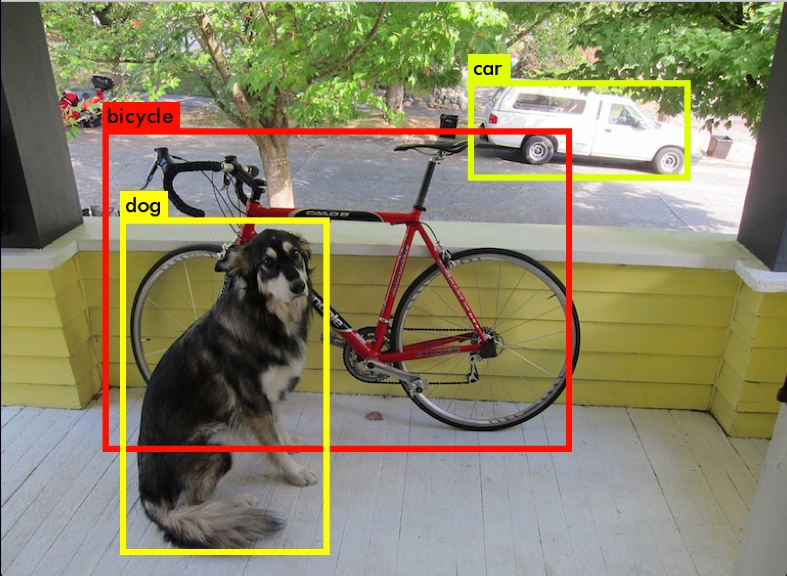
\includegraphics[width=0.5\linewidth]{Image0.jpg}
        \caption{Пример выделения}
        \end{center}
    \end{figure}

	
	Метрикой, которая будет дальше чаще всего встречаться является Mean Average Precision, но сначала опишем, как считать успешность детекции. Так как выделение точного bounding box является слишком сложной и бессмысленной задачей, для определения удачности детектирования будет считаться следующая  метрика, по предсказанному и базовому расположению объекта $IoU = \frac{Area of Overlap}{Area of Union}$. Соответветсвенно, если $IoU > p$, некоторой границы, будем считать что объекты сматчены. Далее проверяется совпадение классов. Далее для подсчета MAP сортируем предсказания в соответсвии с уверенностью модели. Далее считаем precision и recall на всех префиксах этого множества. Тогда $MAP = \frac{1}{|recalls|}\sum\limits_{i=1}^{|recalls|} max(precision(recall) * I(recall >= recalls_i))$ В качестве примера реколы можно выбрать как $0;0.1 ... 1$
	\section{Описаниие архитектуры и применения}
	В модели есть несколько важных частей.
	\begin{enumerate}
	    \item Генератор гипотез
	    \item Сверточная нейросеть
	    \item Классификатор SVM
	\end{enumerate}
	\begin{figure}[H]
	    \begin{center}
        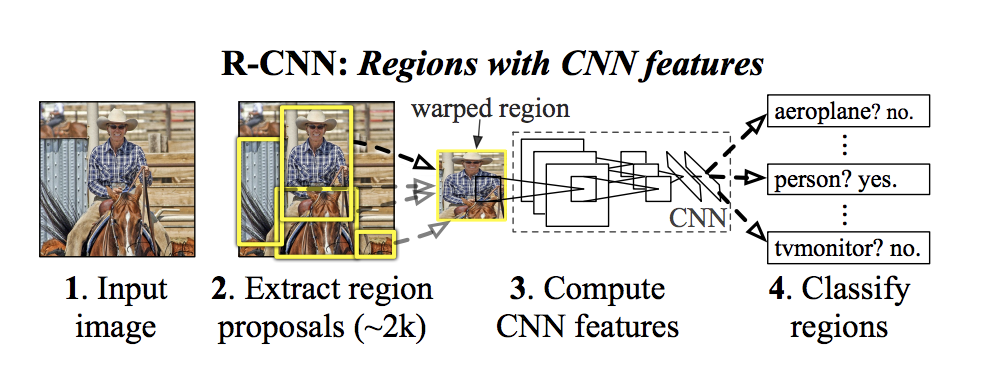
\includegraphics[width=0.8\linewidth]{Image1.png}
        \caption{Демонстрация работы модели по шагам}
        \end{center}
    \end{figure}
    \subsection{Генератор гипотез}
	В качестве генератора гипотез в модели R-CNN используется алгоритм selective search. Он не является обучаемым. В нем генерируется 2000 гипотез объектов на изображении.
	\subsection{Сверточная нейросеть}
	Сверточная нейросеть используется для извлечения фичей из гипотез выделенных selective search. Для этого каждая гипотеза приводится к размеру, который принимает на вход сеть, фичами же являются выходные знаечения последнего слоя сети(полносвязного). В оригинальной статье использовали архитектуру AlexNet. 
	\begin{figure}[H]
	    \begin{center}
        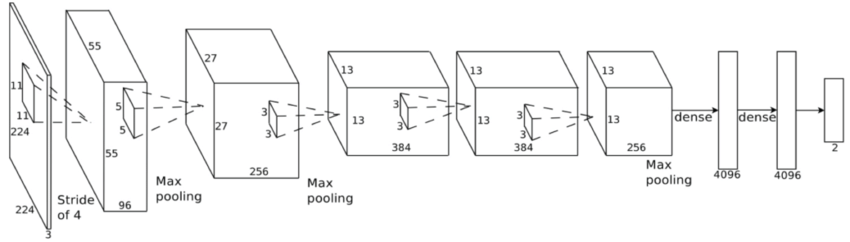
\includegraphics[width=0.8\linewidth]{AlexNet.png}
        \caption{Архитектура AlexNet}
        \end{center}
    \end{figure}
    В дальнейшем в данной модели использовали и другие архитектуры, которые хорошо показали себя в классификации, например, VGG. Более новые архитектуры не использовались, в связи с тем, что были выпущены качественные улучшения данной модели. При этом сверточная нейросеть используется предобученная для задачи классификации.
    \subsection{SVM}
    Для определения класса, к которому относится объект используется линейный классификатор SVM. Также для более повышения качетсва детектирования, производится регрессия границ bounding box. Победивший класс определяется по наибольшей уверенности, среди всех. Для обучения необходимо обучить всего одну матрицу. Авторы утверждают, что SVM был добавлен ими, так как они не хотели файнтюнить сверточную сеть, чтобы вставить в нее softmax, однака даже с файнтюнингом, качество softmax добаленного прямо к нейросети было ниже.
	\section{Особенности обучения}
	В обучении этой  архитектуры можно выделить следующие интересные пункты
	\begin{enumerate}
	    \item Сверточная нейросеть сначала обучается для задачи классификации изображений ImageNet.
	    \item Затем нейросеть доучивают для задачи детекции, подавая только корректные bounding box из training set датасета для детекции с соответствующим классом.
	    \item Изначально SVM обучают с правильными примерами и случайными в качестве негативных. Затем произодится дополнительная добыча негативных примеров из наиболее уверенных ошибок детекции.
	    \item Для увеличения размера обучающей выборки к правильным примерам добавляют также немного сдвинутые их версии.
	\end{enumerate}
	\section{Результаты работы}
	В качестве валидационного  датасета использовался датасет  PASCAL-VOC2007 и 2010.
	Бейзлайном выступала DPM модель на основе гистограм градиентов(HoG).
	\begin{table}[H]
	    \centering
	    \begin{tabular}{|c|c|c|}
	    \hline
	         Модель & VOC-2007 & VOC-2010  \\ \hline
	         DPM & 33.7 & 29.6  \\ \hline
	         R-CNN(only cnn) & 54.2 & 50.2  \\ \hline
	         R-CNN(full) & 58.5 & 53.7  \\ \hline
	         R-CNN(VGG) & 66.0 & 62.9  \\ \hline
	    \end{tabular}
	    \caption{Сравнение моделей}
	\end{table}
	
	\section{Достоинства и недостатки}
	\subsection{Достоинства}
	На момент выхода эта модели показывала наилучшее качество в задаче обнаружения объектов на ихобраэении, так как она одна из первых максимально использовала весь потенциал сверточных нейросетей, которые уже держали лидирующие места в задачи классификации изображений. 
	\subsection{Недостатки}
	\begin{enumerate}
	    \item Очень долго занимает применение сети для одного изображения ~48 секунд. 
	    \item Качество детекции сильно ограничено качеством selective search, так как он не обучаемый.
	    \item Много времени уходит на обучение 84 часа.
		\end{enumerate}

	\section{Краткий обзор улучшений}
	\subsection{Fast R-CNN}
	Одной из главные проблем R-CNN является применение нейросети к каждой гипотезе, это занимает достаточно продолжительное время. В этой архитектуре сеть применяется только один раз ко всему изображению. На первом этапе используется полносверточная сеть, гипотезы же выделяются анологично обычной R-CNN, далее эти гипотезы при помощи RoI pooling слоя, выделяются фичи соответствующие этим гипотезам, и эти вектора подаются в полносвязные слои на выходе нейросети, их которых мы получаем предсказание класса гипотезы и границы, при помощи регрессии. Этой архитектуре требуется в 10 раз меньше времени на обучение и в 20 раз меньше времени на применении. Качество обнаружения при этом увеличивается примерно на 10\%.
	\begin{figure}[H]
	    \begin{center}
        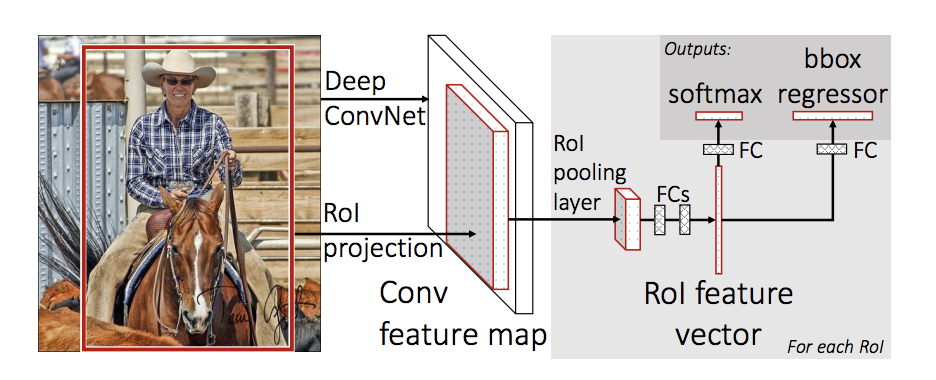
\includegraphics[width=0.8\linewidth]{Fast.png}
        \caption{Архитектура Fast R-CNN}
        \end{center}
    \end{figure}
	
	В данной архитектуре скорость применения ограничивается уже не применением нейросети, а работой selective search.
	\subsection{Faster R-CNN}
	В данной модели отказались от selective search, как генератора гипотез. Весь процесс аналогичен Fact R-CNN, но предсказания гипотез делает отдельная нейросеть, которая обучается на фичах, полученных от полносверточной сети. Такое изменение позволило довести скорость работы почти до реального времени 5 кадров в секунду. 
	\begin{figure}[H]
	    \begin{center}
        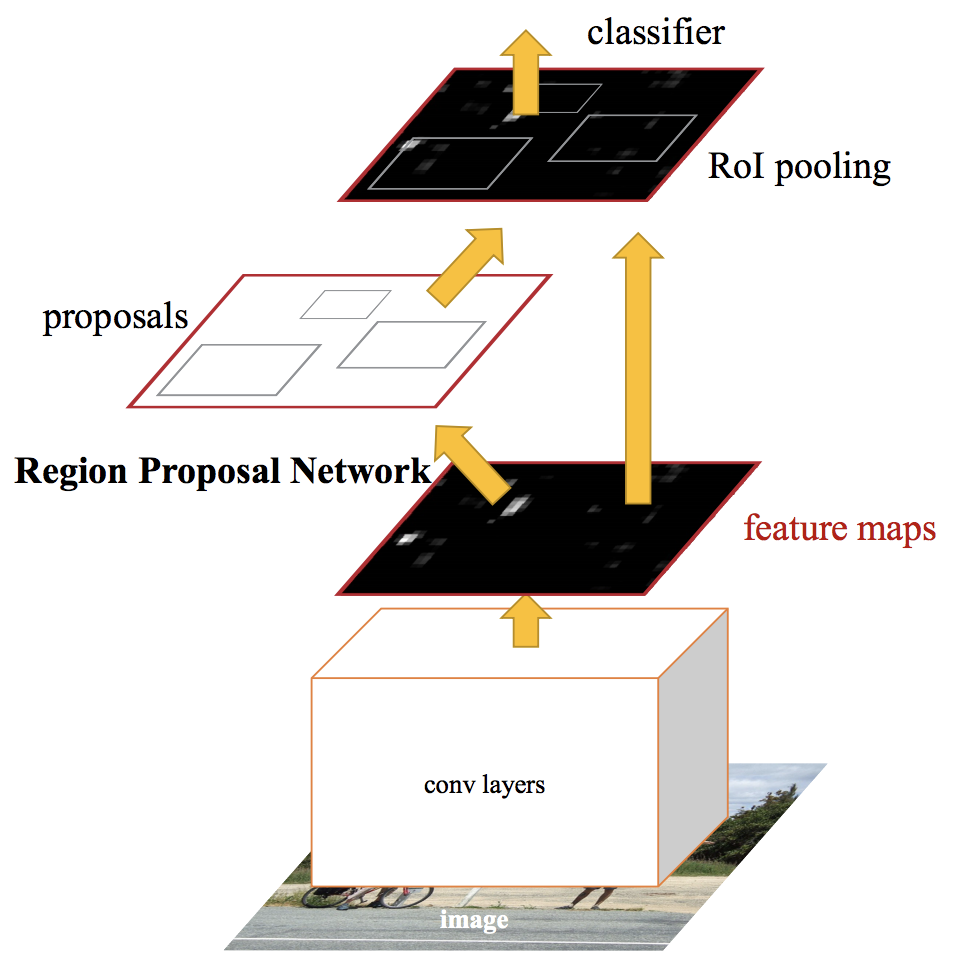
\includegraphics[width=0.4\linewidth]{Faster.png}
        \caption{Архитектура Faster R-CNN}
        \end{center}
    \end{figure}
	
\end{document}